\section{Parse Generators \& Grammar Types}


Lexical analysis and parsing are closely linked to 
compiler design. Though instead of writing such parsers by 
hand, we will use \textbf{parser generators}:

\begin{Def}[Parser Generators]

    \label{def:parser-generator}
    Parser generators are programs that take a representation of formal grammar as input and produces a parser as output.
\end{Def}

\noindent
We'll use \textbf{Menhir} for OCaml. There are other options but this suffices for our needs.
\begin{Def}[Menhir]

    Menhir is an LR(1) parser generator for OCaml. LR(1) stands for:
    \begin{itemize}
        \item \textbf{L}: Left-to-right scanning of the input.
        \item \textbf{R}: Rightmost derivation in reverse. Meaning, it builds the parse tree from the leaves up to the root.
        \item \textbf{(1)}: One symbol of lookahead. This means that the parser can look at one token ahead in the input stream to make parsing decisions.
    \end{itemize}
    \noindent
    Users input small OCaml snippets to define the production rules of the grammar.
\end{Def}

\newpage 

\noindent
A quick aside on Domain Specific Languages (DSLs):

\begin{Def}[Domain Specific Language (DSL)]

    A domain-specific language (DSL) is a programming language or specification language dedicated to a particular problem domain.
    An example of a DSL is SQL, as its only purpose is to query databases. This is in contrast to general-purpose languages like Python, which can be used for a wide range of applications.

    DSL's require custom parsers to be written. This can be done by hand, or using parser generators.
\end{Def}

\noindent
Now we discuss \textbf{Extended BNF (EBNF)}, which allows us to be more expressive in our grammars with less noise.

\begin{Def}[Extended BNF (EBNF)]

\label{def:ebnf}
Extended Backus-Naur Form (EBNF) is a notation for specifying formal grammars, building upon BNF (Backus-Naur Form) by introducing syntactic extensions for greater clarity and brevity.
EBNF includes the following additional constructs:

\begin{itemize}
    
    \item \texttt{|} — alternation: denotes choice between patterns.
    \begin{itemize}
        \item \textbf{E.g.,}  \snippet{<letter> ::= A | B | C}, means that <letter> can be A, B, or C.
    \end{itemize}
    \item \texttt{\{\ldots \}} — repetition: the enclosed pattern may repeat \underline{\textbf{zero} or more times}.
    \begin{itemize}
        \item \textbf{E.g.,}  \snippet{<digits> ::= \{0 | 1 | 2 | 3 | 4 | 5 | 6 | 7 | 8 | 9\}}, match:
        \begin{itemize}
            \item[>] \texttt{"0"}, \texttt{"320"}, \texttt{"11235813"}
        \end{itemize}
    \end{itemize}
    \item \texttt{[\ldots ]} — optionality: the enclosed pattern may appear zero or one time.
    \begin{itemize}
        \item \textbf{E.g.,} \snippet{<number> ::= ["-"] <digits>}, match:
        \begin{itemize}
            \item[>] \texttt{"1"}, \texttt{"-320"}
        \end{itemize}
    \end{itemize}
    \item \texttt{(\ldots )} — grouping: used to group sequences or alternatives.
    \begin{itemize}
        \item \textbf{E.g.,} \snippet{<sum> ::= <number> {("+" | "-") <number>}}, matches:
        \item [>] \texttt{"1 + 2 - 3"}, \texttt{"-1 + 2"}, \texttt{"5"}
        \end{itemize}
    \item \texttt{"\ldots"} — terminal strings may be written in quotes. This clears ambiguity between terminal and non-terminal symbols.
    \begin{itemize}
        \item \textbf{E.g.,} in \snippet{<digit> ::= A | B | C}, it's clear that A, B, and C refer to non-terminal symbols. However, in the expression \snippet{<expr> ::= <expr> | "(" <expr> ")"}, the parenthesis are \textbf{crucial} in indicating that it is not grouping notation.
    \end{itemize}
\end{itemize}
\end{Def}

\newpage

Let's elaborate more on \snippet{<digits>} from above:
\begin{Example}[Dealing with Optionality]

    In our previous grammar from Definition (\ref{def:ebnf}), we had:
    \begin{lstlisting}[numbers=none]
        <digit> ::= {0 | 1 | 2 | 3 | 4 | 5 | 6 | 7 | 8 | 9}
    \end{lstlisting}
    which matched:
    \begin{itemize}
        \item[>] \texttt{"0"}, \texttt{"320"}, \texttt{"11235813"}
    \end{itemize}

    \noindent
    But also unintentionally matched:
    \begin{itemize}
        \item[>] \texttt{""} \hfill \textit{(empty string)}
        \item[>] \texttt{"000"}, \texttt{"0123"} \hfill \textit{(leading zeros)}
    \end{itemize}
    
    \noindent
    Let's first fix the empty string case:
    \begin{lstlisting}[numbers=none]
        <digit> ::= 0 | 1 | 2 | 3 | 4 | 5 | 6 | 7 | 8 | 9
        <digits> ::= <digit> {<digit>}
    \end{lstlisting}

    \noindent
    To restrict leading zeros (e.g., for natural numbers), we refine further:
    \begin{lstlisting}[numbers=none]
        <nonzero> ::= 1 | 2 | 3 | 4 | 5 | 6 | 7 | 8 | 9
        <digits> ::= "0" | <nonzero> {<digit>}
    \end{lstlisting}

    \noindent
    Adding quotes around \snippet{0} is a stylistic choice and does not change the meaning of the grammar. We could have written:
    \begin{lstlisting}[numbers=none]
        <nonzero> ::= "1" | "2" | "3" | "4" | "5" | "6" | "7" | "8" | "9"
        <digits> ::= "0" | <nonzero> {<digit>}
    \end{lstlisting}
    \noindent
    Or without quotes, it doesn't matter as long as there is no ambiguity.
\end{Example}

\noindent
To be more precise with our language we briefly discuss \textbf{Automata Theory} and types of grammars:

\begin{Def}[Automata Theory]

    In mathematics, an automaton (Plural form: automata) is an abstract machine that follow a sequence of states (similar to a 
    flowchart). A finite number of states describe a \textbf{finite automaton (FA)} or \textbf{finite-state machine (FSM)}.
    \end{Def}

\begin{Tip}
    Automata comes from the Greek word $\alpha\upsilon\tau\acute{o}\mu\alpha\tau o\varsigma$ (autómatos), which means ``self-acting, self-willed, self-moving"
\end{Tip}

\newpage 


\noindent
Consider the following automaton described by a state machine diagram:

\begin{figure}[h]
    \centering
    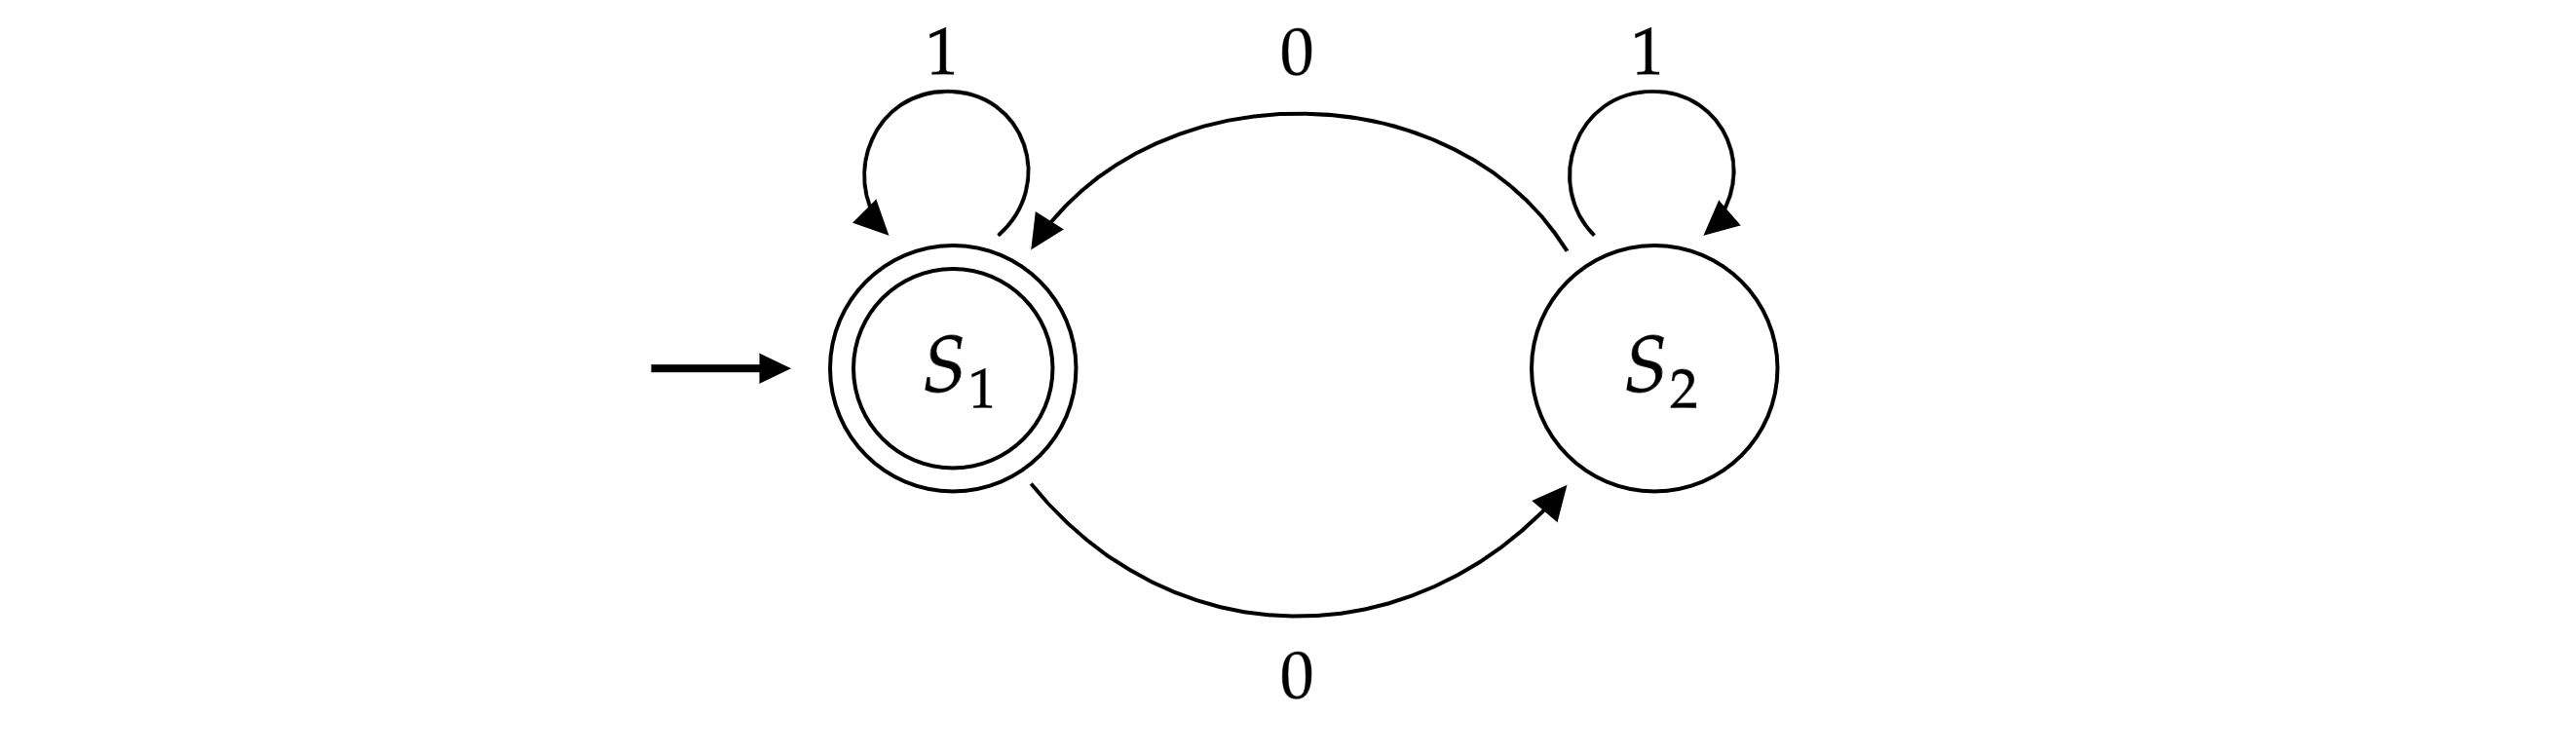
\includegraphics[width=\textwidth]{Sections/Parse/state.png}
    \caption{An automaton represented as a state-machine diagram. This state-machine generates binary strings with an even number of 0's.
    There are two states, $S_1$ and $S_2$. The automaton starts in state $S_1$ as shown by the arrow coming from blank space. The double
    circle indicates the \textbf{accepting state}, at which the automaton may terminate.}
    \label{fig:fa}
\end{figure}

\begin{Def}[Grammar Types]

    In formal language theory, grammars are classified into a hierarchy based on their generative power. This classification, known as the \textbf{Chomsky hierarchy}, comprises four primary types that utilize BNF:

    \begin{itemize}
        \item \textbf{Type 3: Regular Grammars} \\
        Generate \textbf{regular languages}, which can be recognized by finite automata. These grammars can describe simple flat patterns, but cannot handle nested or recursive structures.

        \item \textbf{Type 2: Context-Free Grammars (CFGs)} \\
        Generate \textbf{context-free languages} and are recognized by pushdown automata. A \textbf{pushdown automaton} is a finite automaton extended with a stack—a Last-In, First-Out (LIFO) memory structure. This allows it to handle nested and recursive structures, such as balanced parentheses.

        \item \textbf{Type 1: Context-Sensitive Grammars} \\
        Generate \textbf{context-sensitive languages} and are recognized by linear bounded automata. A \textbf{linear bounded automaton} is a Turing machine where the tape is limited to a length proportional to the input size. This constraint gives it more power than pushdown automata but less than unrestricted Turing machines.

        \item \textbf{Type 0: Unrestricted Grammars} \\
        Generate \textbf{recursively enumerable languages} and are recognized by Turing machines. These grammars have no restrictions on production rules and can describe any computable language, though some of these languages are undecidable.
    \end{itemize}
\end{Def}

\newpage 

\noindent
We can visualize the Chomsky hierarchy as follows:

\begin{figure}[h]
    \centering
    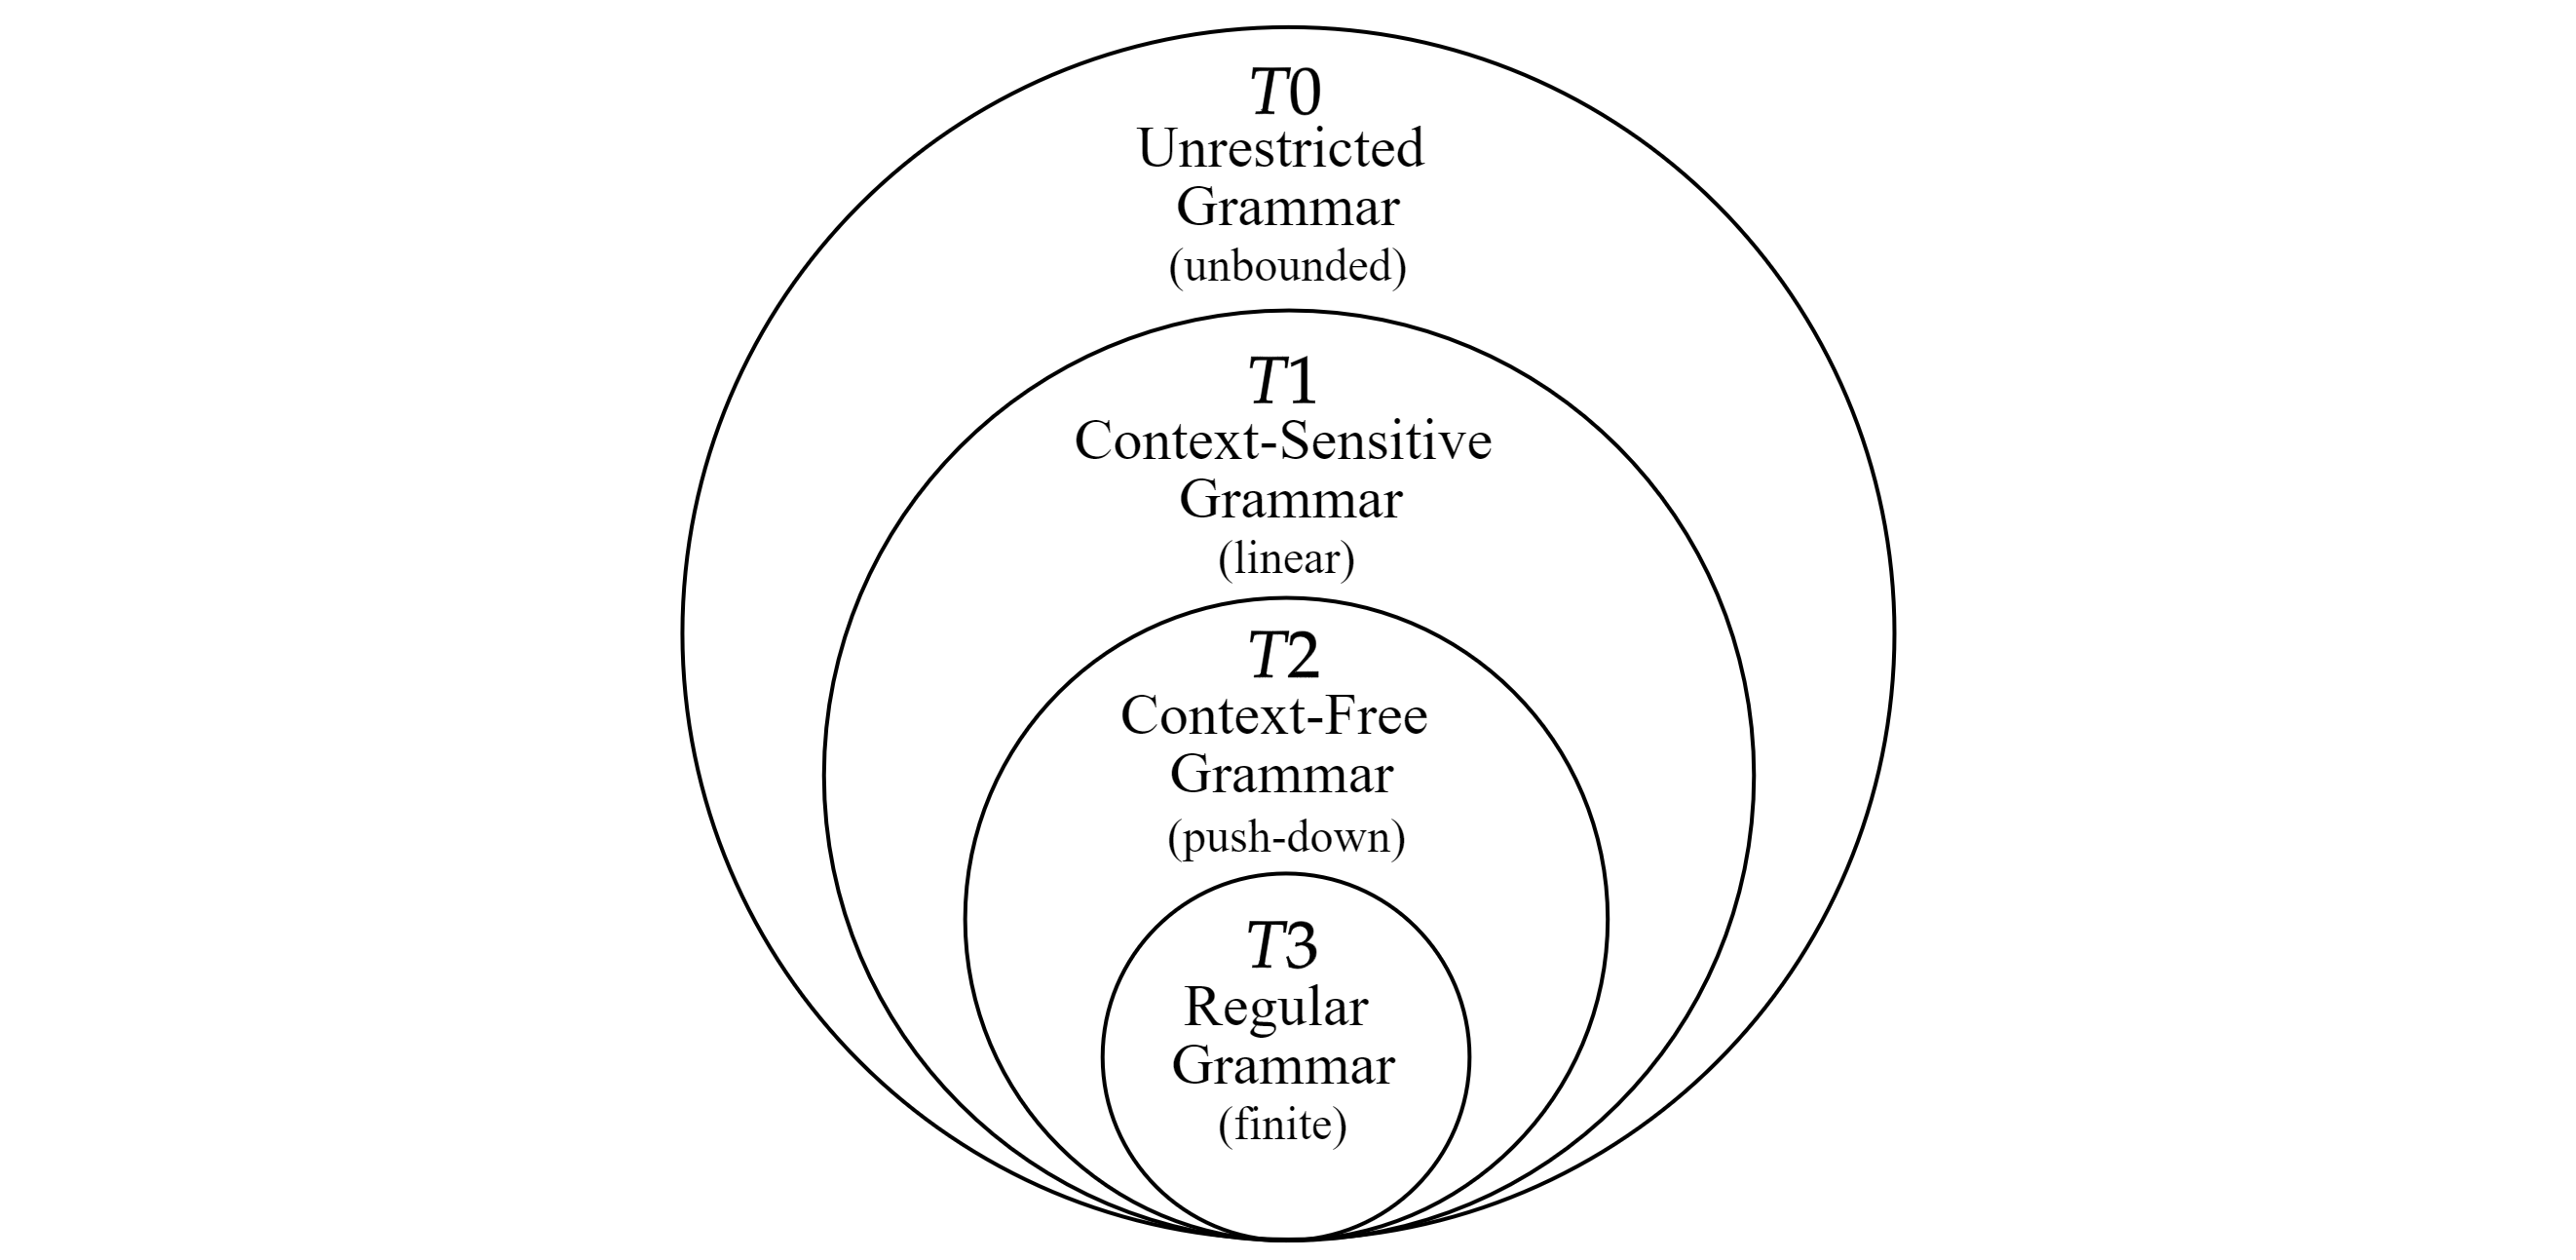
\includegraphics[width=\textwidth]{Sections/Parse/chom.png}
    \caption{
        The Chomsky hierarchy: 
        $T_3$ finite automata (regular expressions), 
        $T_2$ pushdown automata (context-free grammars),
        $T_1$ linear bounded automata (context-sensitive grammars),
        and $T_0$ Turing machines (unrestricted grammars).
    } 
    \label{fig:chomsky}
\end{figure}

\begin{Def}[Regular Expressions (Regex)]

    \label{def:regex}
    Regular expressions (Regex) provide a compact way to describe patterns in regular grammars:
    
    \begin{itemize}
        \item \texttt{a} — a single \textbf{terminal} symbol is itself a regex.
       
    
        \item \texttt{[t1 t2 \ldots tk]} — character class: matches any one of the listed characters.
        
    
        \item \texttt{(e1 | e2 | \ldots | ek)} — alternation: matches any one of the enclosed expressions.
       
    
        \item \texttt{exp*} — repetition: matches \underline{\textbf{zero or more occurrences}} of \texttt{exp}.
      
    
        \item \texttt{exp+} — repetition: matches \underline{\textbf{one or more occurrences}} of \texttt{exp}.
        
    
        \item \texttt{exp?} — optional: matches \underline{\textbf{zero or one occurrence}} of \texttt{exp}.
        
    \end{itemize}
    
    \noindent
    \textbf{E.g.,} the regex \texttt{(a|b)*c} matches any string of a's and b's followed by a c, such as:
    \begin{itemize}
        \item[>] \texttt{"abc"}, \texttt{"aabbbbc"}, \texttt{"c"}
    \end{itemize}
   
    \noindent
    This is just a small subset of the Regex syntax. To learn more, consider the following resource:
    \url{https://regexlearn.com/}
    \end{Def}
    